\section{Method}

\begin{frame}
	\frametitle{Idea}
	
	\Large
	
	\vspace{0.4cm}
	
	\begin{block}{Approach}
		\textbf{Integrate} supervised \textbf{Machine Learning} techniques (e.g., RIPPER, LSQUARE) with
		pure Computer Vision \textbf{feature extractors} (e.g., SIFT, ORB) to \textbf{understand} whether
		a patient \textbf{does have} the Alzheimer disease \textbf{or not} using \emph{Magnetic Resonance
		Imaging} images.
	\end{block}
	
	\vspace{0.2cm}
	
	The method will provide a model which will allow to perform the classification of unseen MRI images,
	thus providing a helpful tool to doctors. \\
\end{frame}

\begin{frame}
	\frametitle{Oriented Fast and Rotated BRIEF (ORB)}
	\framesubtitle{An Example}
	
	\vspace{0.5cm}
	
	\begin{center}
		\begin{figure}[!t]
			\subfigure[Keypoints]
			{
				\begin{tikzpicture}[map/.style={draw=black,ultra thick,inner sep=0pt}]
					\node at (0,0) [map]
					{
						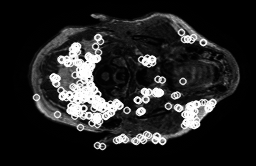
\includegraphics[height=5cm]{Figures/Keypoints}
					};
				\end{tikzpicture}
			}
			\hspace{-0.3cm}
			\subfigure[Descriptors]
			{
				\begin{tikzpicture}[map/.style={draw=white,ultra thick,inner sep=0pt}]
					\node at (0,0) [map]
					{
						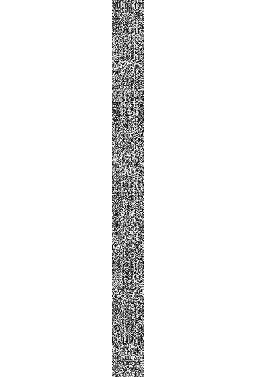
\includegraphics[height=5cm]{Figures/Descriptors}
					};
				\end{tikzpicture}
			}
		\end{figure}
	\end{center}
\end{frame}

\begin{frame}
	\frametitle{Datasets}
	\framesubtitle{Alzheimer's Disease Neuroimaging Initiative}
	
	\Large
	
	\textbf{ADNI}\footnote{\url{http://adni.loni.usc.edu}} is an ongoing study designed to develop
	clinical, imaging, genetic and biochemical biomarkers for the early detection and tracking of
	Alzheimer's disease.
	
	\vspace{0.15cm}
	
	The size of the data set is around 100 GB.
	
	\vspace{0.15cm}
	
	The ADNI began in 2004 with 400 subjects with MCI, 200 with early AD and 200 elderly control
	subjects.\\
	
	\vspace{0.15cm}
	
	In 2011, ADNI2 began assessing participants from the ADNI1/ADNI GO cohort in addition to new
	participants: 150 elderly controls, 100 EMCI, 150 LMCI and 150 AD. \\
\end{frame}

\begin{frame}
	\frametitle{Objective}
	
	\Large
	
	\vspace{0.3cm}
	
	The \textbf{aim} of this research is to \textbf{provide} a tool which can \textbf{help} doctors in
	\textbf{understanding} the evolution of the Alzheimer disease that is the most common form of
	dementia and it is rapidly affecting more patients worldwide.
	
	\vspace{0.4cm}
	
	The proposed approach could be \textbf{extended} for allowing the possibility to \textbf{predict}
	the conversion from MCI or CN to AD by analysing the relation between the models generated for each
	category. \\
\end{frame}
